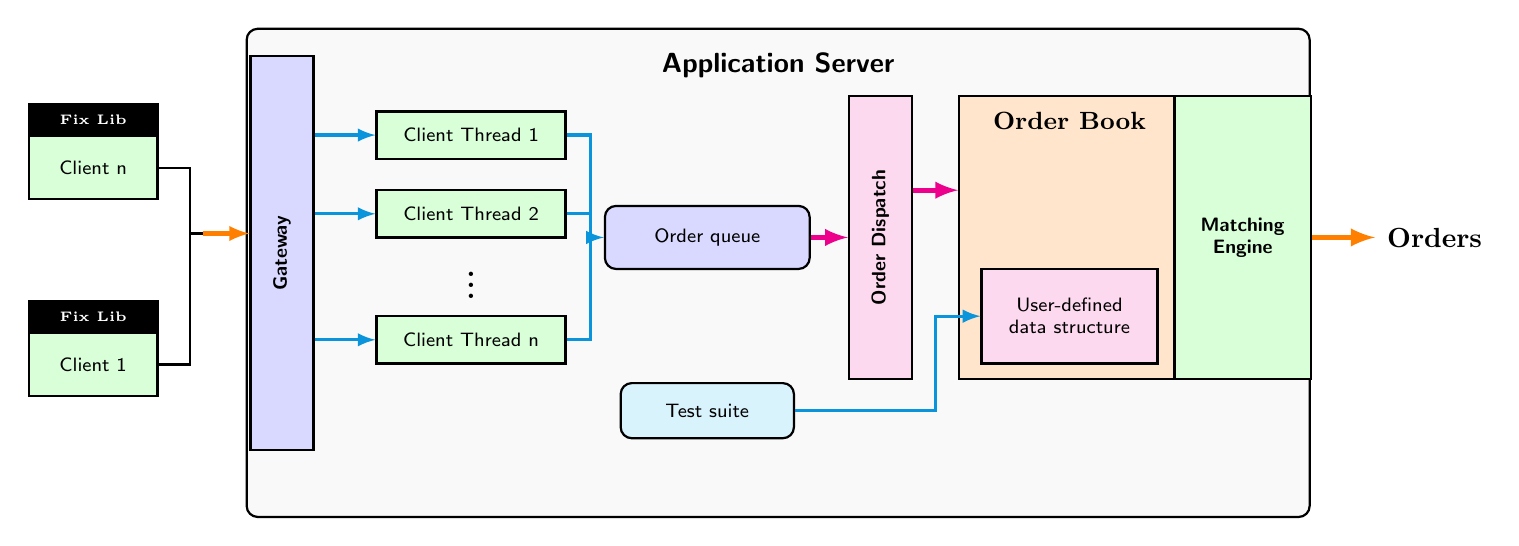
\begin{tikzpicture}[
    >=latex,
    font=\sffamily\scriptsize,
    box/.style={rectangle, draw=black, thick, text centered},
    rbox/.style={rectangle, draw=black, thick, text centered, rounded corners},
    clientnode/.style={box, fill=green!15, text width=1.4cm, minimum height=0.8cm},
    clienthdr/.style={box, fill=black, text=white, text width=1.4cm, minimum height=0.4cm, font=\tiny\bfseries},
    gateway/.style={box, fill=blue!15, minimum width=0.8cm, minimum height=5cm},
    thread/.style={box, fill=green!15, minimum width=2.4cm, minimum height=0.6cm},
    queue/.style={rbox, fill=blue!15, minimum width=2.6cm, minimum height=0.8cm},
    dispatch/.style={box, fill=magenta!15, minimum width=0.8cm, minimum height=3.6cm},
    obbox/.style={box, fill=orange!20, minimum width=2.8cm, minimum height=3.6cm},
    udd/.style={box, fill=magenta!15, text width=2cm, minimum height=1.2cm},
    testuite/.style={rbox, fill=cyan!15, minimum width=2.2cm, minimum height=0.7cm},
    matching/.style={box, fill=green!15, text width=1.5cm, minimum height=3.6cm},
    appserver/.style={rbox, fill=gray!5, minimum width=13.5cm, minimum height=6.2cm}
]

    % 1. Application Server Background
    \node[appserver] (server) at (8.7, -0.25) {};
    \node[font=\sffamily\bfseries\normalsize, anchor=north, yshift=-0.2cm] at (server.north) {Application Server};

    % 2. External Clients
    \node[clientnode, anchor=north] (cn) at (0, 1.5) {Client n};
    \node[clienthdr, anchor=south, yshift=-0.5pt] (cnh) at (cn.north) {Fix Lib};
    \node[clientnode, anchor=north] (c1) at (0, -1.0) {Client 1};
    \node[clienthdr, anchor=south, yshift=-0.5pt] (c1h) at (c1.north) {Fix Lib};

    % 3. Gateway
    \node[gateway] (gw) at (2.4, 0) {\rotatebox{90}{\textbf{Gateway}}};

    % Arrow: Clients to Gateway
    \coordinate (cmid) at (1.4, 0.25);
    \draw[thick] (cn.east) -- ++(0.4,0) |- (cmid);
    \draw[thick] (c1.east) -- ++(0.4,0) |- (cmid);
    \draw[thick, ->, draw=orange, line width=1.5pt] (cmid) -- (gw.west |- cmid);

    % 4. Threads
    \node[thread] (t1) at (4.8, 1.5) {Client Thread 1};
    \node[thread] (t2) at (4.8, 0.5) {Client Thread 2};
    \node[font=\bfseries] at (4.8, -0.3) {\vdots};
    \node[thread] (tn) at (4.8, -1.1) {Client Thread n};

    % Arrows: Gateway to Threads
    \draw[thick, ->, draw=cyan!80!blue, line width=1.2pt] (gw.east |- t1.west) -- (t1.west);
    \draw[thick, ->, draw=cyan!80!blue, line width=1.2pt] (gw.east |- t2.west) -- (t2.west);
    \draw[thick, ->, draw=cyan!80!blue, line width=1.2pt] (gw.east |- tn.west) -- (tn.west);

    % 5. Order Queue
    \node[queue] (oq) at (7.8, 0.2) {Order queue};

    % Arrows: Threads to Queue
    \coordinate (qmid) at (6.3, 0.2);
    \draw[thick, draw=cyan!80!blue, line width=1.2pt] (t1.east) -- ++(0.3,0) |- (qmid);
    \draw[thick, draw=cyan!80!blue, line width=1.2pt] (t2.east) -- ++(0.3,0) |- (qmid);
    \draw[thick, draw=cyan!80!blue, line width=1.2pt] (tn.east) -- ++(0.3,0) |- (qmid);
    \draw[thick, ->, draw=cyan!80!blue, line width=1.2pt] (qmid) -- (oq.west);

    % 6. Order Dispatch
    \node[dispatch] (disp) at (10, 0.2) {\rotatebox{90}{\textbf{Order Dispatch}}};
    \draw[thick, ->, draw=magenta, line width=1.8pt] (oq.east) -- (disp.west);

    % 7. Order Book
    \node[obbox] (ob) at (12.4, 0.2) {};
    \node[font=\bfseries\small, anchor=north, yshift=-0.1cm] at (ob.north) {Order Book};
    \node[udd, anchor=south, yshift=0.2cm] (udd) at (ob.south) {User-defined\\data structure};
    \draw[thick, ->, draw=magenta, line width=1.8pt] (disp.east |- 0, 0.8) -- (ob.west |- 0, 0.8);

    % 8. Test Suite
    \node[testuite] (ts) at (7.8, -2.0) {Test suite};
    \draw[thick, ->, draw=cyan!80!blue, line width=1.2pt] (ts.east) -| (10.7, -1.0) |- (udd.west);

    % 9. Matching Engine
    \node[matching] (me) at (14.6, 0.2) {\textbf{Matching}\\\textbf{Engine}};

    % 10. Output Orders
    \draw[thick, ->, draw=orange, line width=2pt] (me.east) -- ++(0.8,0) node[right, font=\bfseries, text=black] {Orders};

\end{tikzpicture}
